%%%%%%%%%%%%%%%%%%%%%%%%%%%%%%%%%%%%%%%%%
% Beamer Presentation
% LaTeX Template
% Version 1.0 (10/11/12)
%
% This template has been downloaded from:
% http://www.LaTeXTemplates.com
%
% License:
% CC BY-NC-SA 3.0 (http://creativecommons.org/licenses/by-nc-sa/3.0/)
%
%%%%%%%%%%%%%%%%%%%%%%%%%%%%%%%%%%%%%%%%%

%----------------------------------------------------------------------------------------
%   PACKAGES AND THEMES
%----------------------------------------------------------------------------------------

\documentclass{beamer}
%\documentclass[notes=only]{beamer}

\mode<presentation> {

    % The Beamer class comes with a number of default slide themes
    % which change the colors and layouts of slides. Below this is a list
    % of all the themes, uncomment each in turn to see what they look like.

    %\usetheme{default}
    %\usetheme{AnnArbor}
    %\usetheme{Antibes}
    %\usetheme{Bergen}
    %\usetheme{Berkeley}
    %\usetheme{Berlin}
    %\usetheme{Boadilla}
    %\usetheme{CambridgeUS}
    %\usetheme{Copenhagen}
    %\usetheme{Darmstadt}
    %\usetheme{Dresden}
    %\usetheme{Frankfurt}
    %\usetheme{Goettingen}
    %\usetheme{Hannover}
    %\usetheme{Ilmenau}
    %\usetheme{JuanLesPins}
    %\usetheme{Luebeck}
    \usetheme{Madrid}
    %\usetheme{Malmoe}
    %\usetheme{Marburg}
    %\usetheme{Montpellier}
    %\usetheme{PaloAlto}
    %\usetheme{Pittsburgh}
    %\usetheme{Rochester}
    %\usetheme{Singapore}
    %\usetheme{Szeged}
    %\usetheme{Warsaw}

    % As well as themes, the Beamer class has a number of color themes
    % for any slide theme. Uncomment each of these in turn to see how it
    % changes the colors of your current slide theme.

    %\usecolortheme{albatross}
    %\usecolortheme{beaver}
    %\usecolortheme{beetle}
    %\usecolortheme{crane}
    %\usecolortheme{dolphin}
    %\usecolortheme{dove}
    %\usecolortheme{fly}
    %\usecolortheme{lily}
    %\usecolortheme{orchid}
    %\usecolortheme{rose}
    %\usecolortheme{seagull}
    %\usecolortheme{seahorse}
    %\usecolortheme{whale}
    %\usecolortheme{wolverine}

    %\setbeamertemplate{footline} % To remove the footer line in all slides uncomment this line
    %\setbeamertemplate{footline}[page number] % To replace the footer line in all slides with a simple slide count uncomment this line

    %\setbeamertemplate{navigation symbols}{} % To remove the navigation symbols from the bottom of all slides uncomment this line
}

\usepackage{graphicx} % Allows including images
\usepackage{amsmath}
\usepackage{amssymb}
\usepackage{booktabs} % Allows the use of \toprule, \midrule and \bottomrule in tables
\usepackage[utf8]{inputenc}
\usepackage[absolute,overlay]{textpos}

%----------------------------------------------------------------------------------------
%   TITLE PAGE
%----------------------------------------------------------------------------------------

\title[Restore axial resolution CNN]{Restoring axial resolution using a 2D/3D deep convolution neuronal network} % The short title appears at the bottom of every slide, the full title is only on the title page

\author{Joey Zenhäusern} % Your name
\institute[EPFL] % Your institution as it will appear on the bottom of every slide, may be shorthand to save space
{
    \small{
        Section of Computer Science \\
        École Polytechnique Fédérale de Lausanne \\ % Your institution for the title page
        Semester Project -- 12 Credits \\
    }

    \medskip
    Supervision: \\
    Dr. Daniel Sage\\
    Dr. Kyong Jin
}
\date{\today} % Date, can be changed to a custom date

\begin{document}

\begin{frame}
    \titlepage % Print the title page as the first slide
\end{frame}

\begin{frame}
    \frametitle{Overview} % Table of contents slide, comment this block out to remove it
    \tableofcontents % Throughout your presentation, if you choose to use \section{} and \subsection{} commands, these will automatically be printed on this slide as an overview of your presentation
\end{frame}

%----------------------------------------------------------------------------------------
%   PRESENTATION SLIDES
%----------------------------------------------------------------------------------------

%------------------------------------------------
\section{Introduction} % Sections can be created in order to organize your presentation into discrete blocks, all sections and subsections are automatically printed in the table of contents as an overview of the talk
%------------------------------------------------
\begin{frame}
    % PSF is also consequence of mechanical limitations
    % time of aquisition is also a problem when aquiring z slices
    % 100nm vs 1micrometer
    \frametitle{The Problem}
    Due to mechanical limitations in 3D microscopy we have:\\
    \vspace{5pt}
    \begin{center}
        axial resolution (Z) $<<$ lateral resolution (XY)\\
    \end{center}
    \vspace{5pt}
    Traditionally axial resolution is simply interpolated or not changed at all. Anisotropic image data makes downstream 3D image processing much more difficult.\\
    \vspace{10pt}
    Our strategy:\\
    Use a CNN with a U-Net architecture to learn mapping between high and low resolution
    images in XY plane. Then apply learned mapping to Z slices to recover axial resolution.
    % poisson noise and black background
\end{frame}

\begin{frame}
    \frametitle{Processing pipeline}
    \begin{figure}
        \includegraphics[width=\textwidth]{../report/figures/raw_figures/full-pipeline.png}
    \end{figure}
\end{frame}

\section{Methodology}
\subsection{Implementation} % A subsection can be created just before a set of slides with a common theme to further break down your presentation into chunks

\begin{frame}
    \frametitle{The U-Net}
    CNN architecture as presented in Ronneberger et. al \cite{unet}:
    % cite published paper not arxiv
    \begin{itemize}
        \item Contracting path with max pooling \& convolution
        \item Expanding path with upsampling \& convolution
        \item High resolution features from contracting path are combined with upsample layers.
    \end{itemize}
    \begin{figure}
        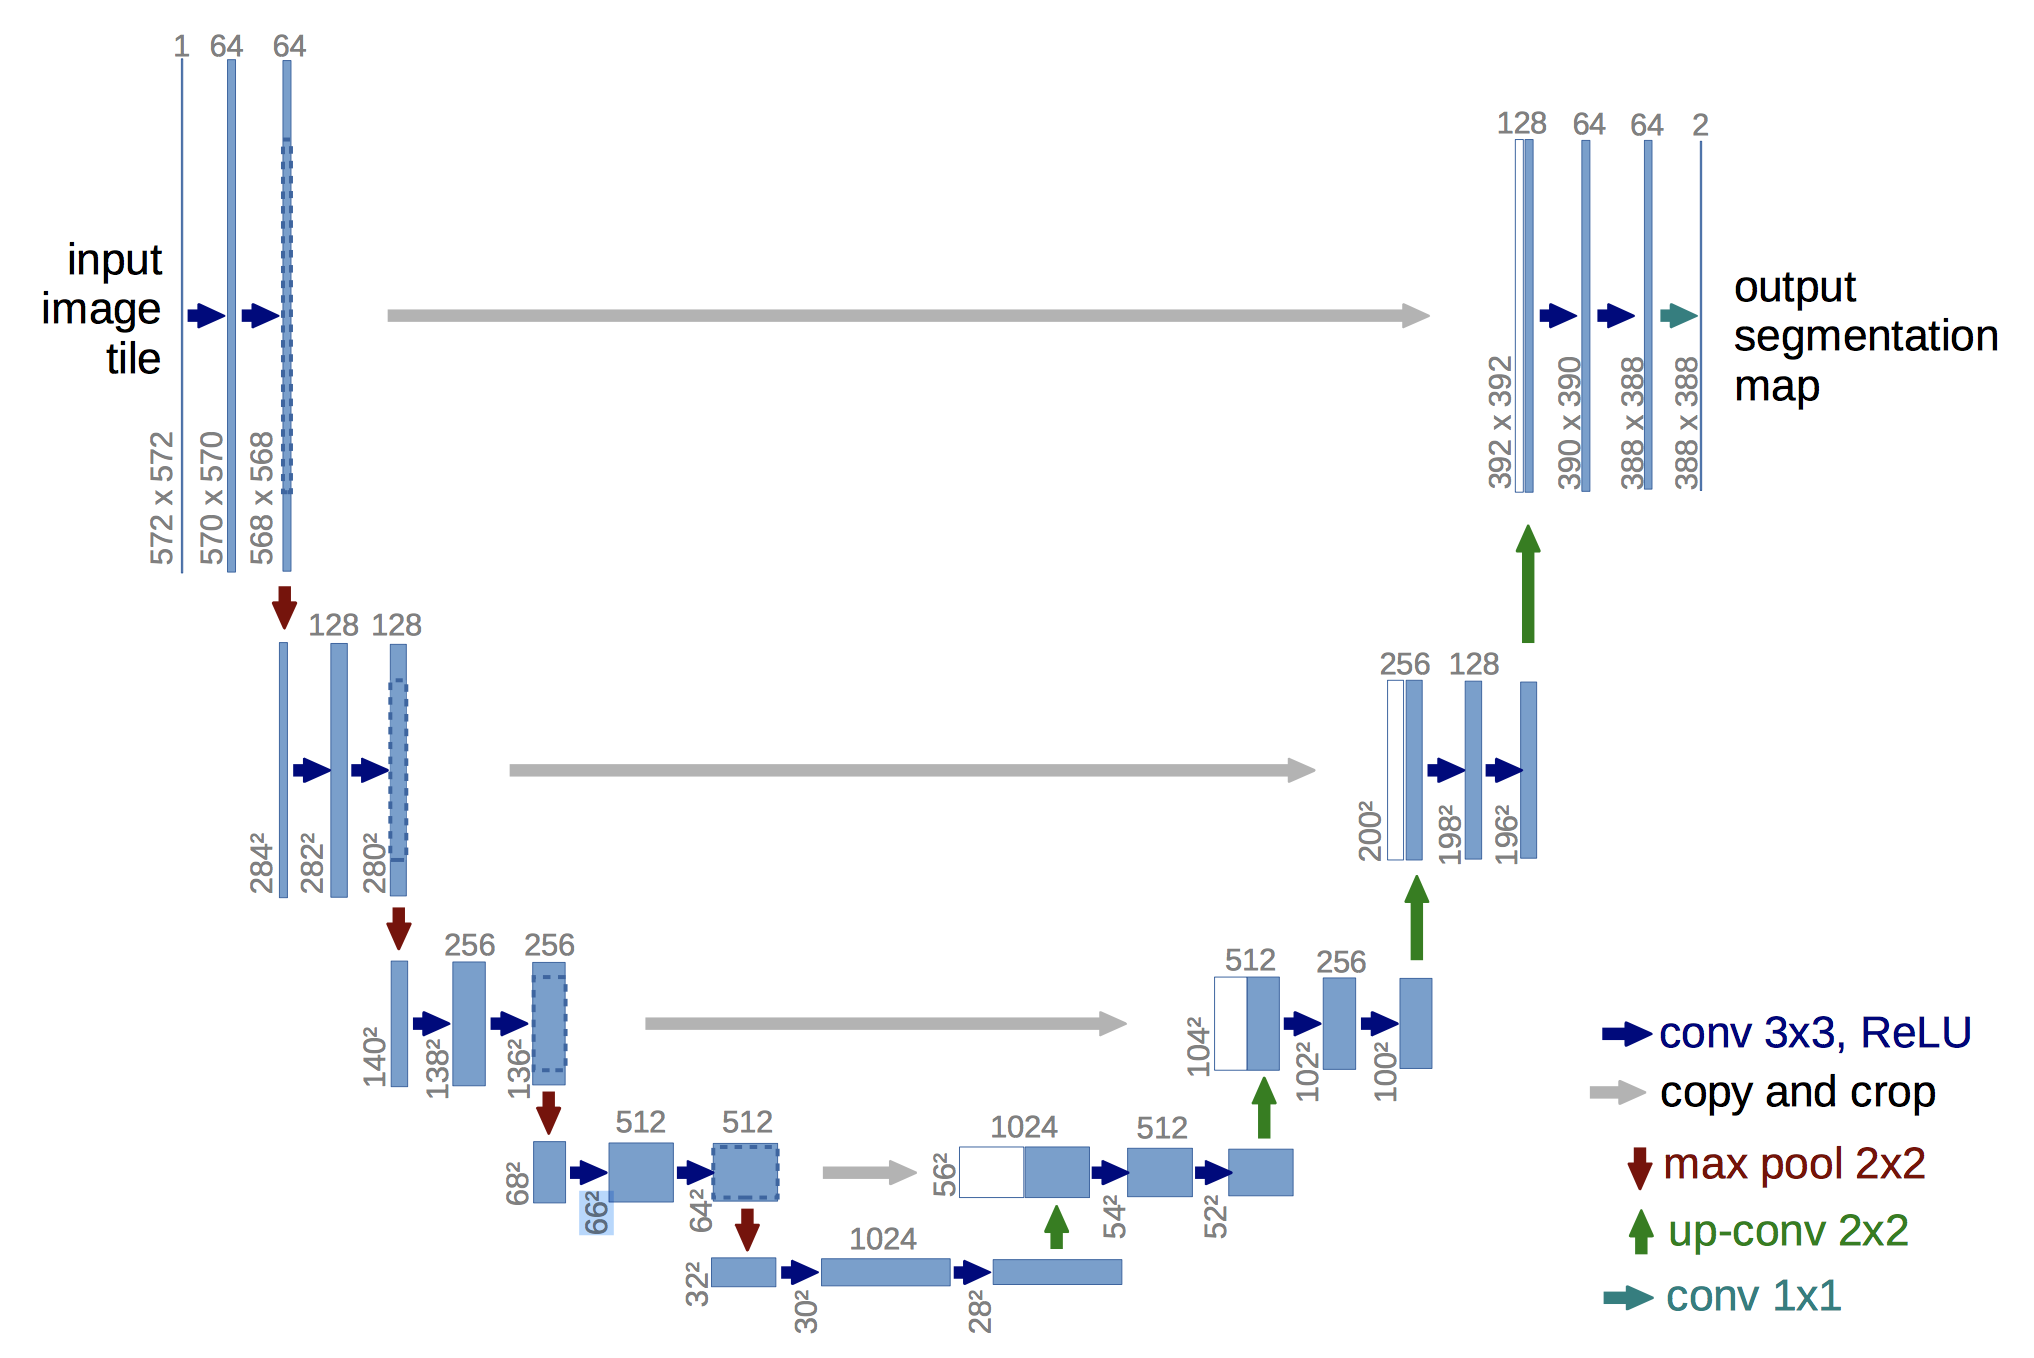
\includegraphics[width=5cm]{../report/figures/unet.png}
    \end{figure}
    \begin{textblock*}{5cm}(7cm,2cm) % {block width} (coords)
    \end{textblock*}

\end{frame}

%------------------------------------------------


\note{
    \begin{itemize}
        \item Explain numlayers, convsize, dilationsize, dropout, kfactor
    \end{itemize}
}

%------------------------------------------------
\begin{frame}
    \frametitle{Training setup}
    Optimization is performed by the Adam optimizer (a more sophisticated version of SGD proposed by Kingma and Ba \cite{kingma2014adam}), which minimizes pixel wise negative PSNR ratio between the ground truth patches ($o(x, y)$) and the predicted patches ($p(x, y)$).
    % mention mse and abs
    \vspace{20pt}
    \begin{block}{Custom Loss function implemented in Tensorflow:}
        \begin{equation}\label{eq:loss}
            \mathcal{L} = -20 \cdot \big[ \log_{10}[\max o(x, y)] - \log_{10}[\sqrt{\text{MSE(o(x, y), p(x, y))}}] \big]
        \end{equation}
    \end{block}
    \vspace{20pt}

    \begin{itemize}
        \item $\max()$: the maximum possible pixel value of the given image.
        \item $\text{MSE()}$: mean squared error between two images.
    \end{itemize}
\end{frame}

\note{
    \begin{itemize}
        \item "Adaptive Moment Estimation"
        \item Maintains learning rate for each network weight individually
        \item State of the Art optimizer
    \end{itemize}
}

%------------------------------------------------

\subsection{Network Architecture}
\subsubsection{Baseline Network}
\begin{frame}
    \frametitle{Baseline U-Net Network}
    % make this clearer
    Based on \textit{Isonet-2}, from Myers et al. \cite{WEIGERT2017}:

    \begin{equation*}
        C_{16, 7} - M_{2} - C_{32, 7} - M_{2} - C_{64, 7} - U_{2} - C_{32, 7} - U_{2} - C_{16, 7} - C_{1, 1}
    \end{equation*}

    \begin{align*}
        C_{n, c}:\quad &\text{Convolutional layer with $n$ filters of size $(c, c)$}\\
        M_{m}:\quad &\text{Max pooling layer with a subsample factor of $(m, m)$}\\
        U_{u}:\quad &\text{Upsampling layer with a subsample factor of $(u, u)$}
    \end{align*}

    We use ReLu activation and zero padding for convolutional layers.
\end{frame}

\note{
    \begin{itemize}
        \item Explain Network notation
        \item (Number of filters is number of neurons, and hence the number of features in the resulting featuremap)
    \end{itemize}
}

\subsubsection{Dilated Convolution}
\begin{frame}
    \frametitle{Dilated Convolution}
    \begin{itemize}
        \item Baseline network uses $(7, 7)$ filters for convolutions: High memory usage and computationally expensive
        \item Dilated convolution can be seen as a Strided convolution
        \item Saves memory while retaining larger receptive field
        \item Goal: Faster training with similar or better results
    \end{itemize}
    \begin{figure}[h]
        \center%
        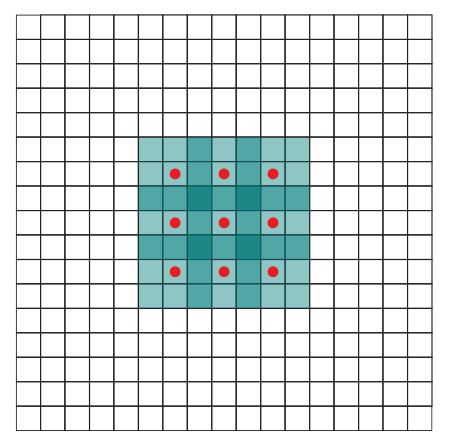
\includegraphics[width=0.3\columnwidth]{../report/figures/dilated.png}
    \end{figure}
\end{frame}

\subsubsection{Increasing Network Depth}
\begin{frame}
    \frametitle{Increase Network Depth}
    \begin{itemize}
        \item Another approach to retain receptive field size while lowering memory and computational cost
        \item Our model can be trained for any depth as long as the patch size can be evenly divided by $2^n$, where $n$ is the number of max pooling layers in the network.
    \end{itemize}
\end{frame}

\subsection{Hyperparameter Optimization}
\begin{frame}
    \frametitle{Hyperparameter Optimization}
    \begin{itemize}
        \item \texttt{learning\_rate}: $10^{-3}$
        \item \texttt{dropout}: Regularization technique that randomly discards neurons in the network in every training iteration.
            \begin{itemize}
                \item + Less likely to overfit
                \item + Potentially better predictions for previously unseen data
                \item - Slower convergence \& training
                \item - Potentially reduced accuracy for predictions
            \end{itemize}
    \end{itemize}
\end{frame}

\begin{frame}
    \frametitle{Main Parameters}
    The behavior of the training routine can easily be controlled by a number of parameters which can be passed as flags when executing the routine.
    \vspace{30pt}
    \begin{columns}[t]
        \column{0.5\textwidth}
            Network parameters
            \begin{itemize}
                \item \texttt{num\_layers}
                \item \texttt{conv\_size}
                \item \texttt{dilation\_size}
                \item \texttt{dropout}
            \end{itemize}
        \column{0.5\textwidth}
            General parameters
            \begin{itemize}
                \item \texttt{patch\_size}
                \item \texttt{stride}
                \item \texttt{k\_factor}
                \item \texttt{num\_epoch}
            \end{itemize}
    \end{columns}
\end{frame}

\section{Results}
\begin{frame}
    \frametitle{Data}
    The dataset used to evaluate the model's performance is synthetic and simulates cells of a c-elegans. There is deterioration through gaussian noise, poisson noise and shape deformation.
    \begin{figure}
        \includegraphics[width=0.4\textwidth]{../report/figures/raw_figures/gt.png}
    \end{figure}
\end{frame}

\begin{frame}
    \frametitle{Model Evaluation Results}
    \begin{columns}[t]
        \column{0.4\textwidth}
        \small
        Parameters equal for all models:
        \begin{itemize}
            \item \texttt{learning\_rate}=$10^{-3}$
            \item \texttt{k\_factor}=3
            \item \texttt{patch\_size}=120
            \item \texttt{stride}=60
        \end{itemize}

        Network parameters:
        \begin{itemize}
            \item d: \texttt{dilation\_size}
            \item c: \texttt{conv\_size}
            \item n: \texttt{num\_layers}
        \end{itemize}
        
        \vspace{10pt}
        \footnotesize
        $\text{PSNR}_i$ is the PSNR increase from groundtruth-bicubic (20.51dB) to groundtruth-prediction.

        \column{0.6\textwidth}
        \begin{table}[h]
            \small
            \centering
            \begin{tabular}{c | c | c | c | c | c | c}
                \#  & d & c & n & dropout & $\text{PSNR}_i$ & time \\
                \hline
                \hline
                1  & -             & 7          & 3           & 0\%     & 1.55        & 82min                                                                    \\
                \hline
                2  & 5             & 3          & 3           & 0\%     & 1.51        & 70min                                                                    \\
                \hline
                3  & 3             & 3          & 3           & 0\%     & 1.50        & 61min                                                                    \\
                \hline
                4  & -             & 3          & 4           & 0\%     & 1.49        & 57min                                                                    \\
                \hline
                5  & -             & 7          & 3           & 10\%     & 0.55       & -                                                                     \\
                \hline
                6  & 5             & 3          & 3           & 10\%     & 0.46       & -                                                                     \\
                \hline
                7  & 3             & 3          & 3           & 10\%     & 0.43       & -                                                                     \\
                \hline
                8  & -             & 5          & 3           & 10\%     & 0.42       & -                                                                     \\
                \hline
                9  & -             & 3          & 4           & 10\%     & 0.37       & -                                                                     \\
                \hline
                10  & -             & 3          & 3           & 10\%     & 0.32      & -                                                                      \\
                \hline
                11  & -             & 5          & 4           & 10\%     & 0.32      & -                                                                      \\
                \hline
                12  & 7             & 3          & 3           & 10\%     & 0.29      & -
            \end{tabular}
            \label{tab:mresults}
        \end{table}
    \end{columns}
\end{frame}

\begin{frame}
    \frametitle{Model 3 visual results}
    Using the previous notation we can express model 3 as follows
    \begin{align*}
        C_{16, 3} - D_{16, 3} - M_{2} - C_{32, 3} - D_{32, 3} - M_{2} - C_{64, 3} - D_{64, 3} \\
        - U_{2} - C_{32, 3} - D_{32, 3} - U_{2} - C_{16, 3} - D_{16, 3} - C_{1, 1}
    \end{align*}
    where
    \begin{align*}
        D_{n, c}:\quad &\text{Dilated convolutional layer with $n$ filters of size $(c, c)$}
    \end{align*}
    \begin{figure}
        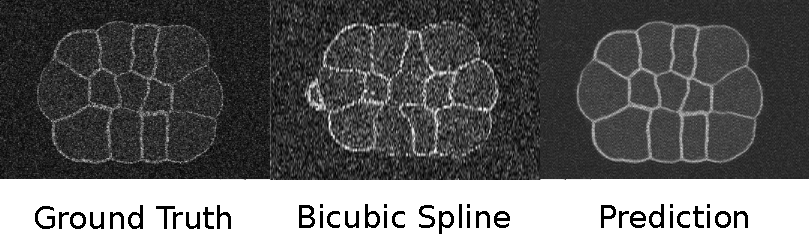
\includegraphics[width=1\textwidth]{../report/figures/better_results.pdf}
    \end{figure}
\end{frame}

\begin{frame}
    \frametitle{Results}
    If we increase the \texttt{k\_factor} we get the following results:
    \vspace{30pt}
    \begin{table}
        \centering
        \begin{tabular}{l | l | l}
            & k\_factor & \begin{tabular}[c]{@{}l@{}}PSNR increase vs.\\ bicubic interpolation (dB)\end{tabular} \\
            \hline
            \hline
            1 & 4         & 1.90                                                                                   \\
            \hline
            2 & 5         & 1.89                                                                                   \\
            \hline
            3 & 6         & 1.95                                                                                  
        \end{tabular}
    \end{table}
\end{frame}

\begin{frame}
    \frametitle{Generated Predictions}
    Visual results for higher k\_factor values:
    \begin{figure}
        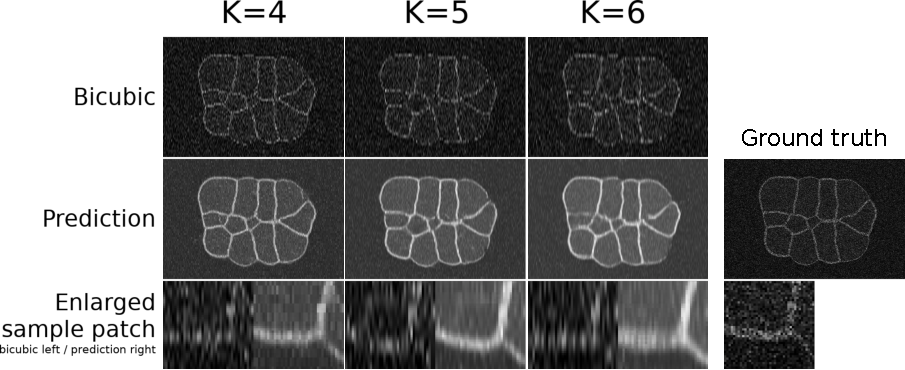
\includegraphics[width=1\columnwidth]{../report/figures/prediction_pres.pdf}
    \end{figure}
\end{frame}

\section{Conclusion}

\begin{frame}
    \frametitle{Conclusion}
    Results show that:
    \begin{itemize}
        \item CNN supperresolution using U-Net is promising
        \item PSNR increase of up to 1.55dB for \texttt{k\_factor} $=3$
        \item PSNR increase around 1.9dB for \texttt{k\_factor} $\in {4, 5, 6}$
        \item Training time can be improved through various architectures while retaining accuracy.
    \end{itemize}

    Possible future extension of this work:
    \begin{itemize}
        \item Take PSF into account for training
        \item Deeper exploration of hyperparameter space and different network architectures
    \end{itemize}
\end{frame}

%------------------------------------------------
\begin{frame}
    \frametitle{References}
    \bibliographystyle{acm}
    \bibliography{../report/report}
\end{frame}

%------------------------------------------------

\begin{frame}
    \Huge{\centerline{Discussion}}
\end{frame}

%----------------------------------------------------------------------------------------

\end{document}
